\thispagestyle{empty}

\noindent
\begin{minipage}[t]{0.27\textwidth}
    \vspace{0pt}
    % Ghi chú lề 1
    \begin{tcolorbox}[
        colback=stewartpurple!8!white,
        colframe=stewartpurple!8!white,
        arc=1mm,
        left=1mm, right=1.5mm, top=1mm, bottom=1mm,
        boxrule=0pt
    ]
        \hangindent=7.5mm\hangafter=1
        \mbox{\colorbox{stewartpurple}{\rule[-0.2ex]{0pt}{1.8ex}\color{white}\scriptsize\textbf{\textsf{\,PS\,}}}}%\hspace{1.5mm}\footnotesize\textsf{Vẽ một hình vẽ.}
    \end{tcolorbox}
    
    \vspace{2.8cm}
    
    % Ghi chú lề 2 & 3
    \begin{tcolorbox}[
        colback=stewartpurple!8!white,
        colframe=stewartpurple!8!white,
        arc=1mm,
        left=1mm, right=1.5mm, top=1mm, bottom=1mm,
        boxrule=0pt
    ]
        \hangindent=7.5mm\hangafter=1
        \mbox{\colorbox{stewartpurple}{\rule[-0.2ex]{0pt}{1.8ex}\color{white}\scriptsize\textbf{\textsf{\,PS\,}}}}%\hspace{1.5mm}\footnotesize\textsf{Liên hệ cái đã cho với cái chưa biết.}
    \end{tcolorbox}
    \vspace{1.5mm}
    \begin{tcolorbox}[
        colback=stewartpurple!8!white,
        colframe=stewartpurple!8!white,
        arc=1mm,
        left=1mm, right=1.5mm, top=1mm, bottom=1mm,
        boxrule=0pt
    ]
        \hangindent=7.5mm\hangafter=1
        \mbox{\colorbox{stewartpurple}{\rule[-0.2ex]{0pt}{1.8ex}\color{white}\scriptsize\textbf{\textsf{\,PS\,}}}}%\hspace{1.5mm}\footnotesize\textsf{Đưa thêm yếu tố phụ.}
    \end{tcolorbox}

    \vspace{6.8cm}

    % Ghi chú lề 4
    \begin{tcolorbox}[
        colback=stewartpurple!8!white,
        colframe=stewartpurple!8!white,
        arc=1mm,
        left=1mm, right=1.5mm, top=1mm, bottom=1mm,
        boxrule=0pt
    ]
        \hangindent=7.5mm\hangafter=1
        \mbox{\colorbox{stewartpurple}{\rule[-0.2ex]{0pt}{1.8ex}\color{white}\scriptsize\textbf{\textsf{\,PS\,}}}}%\hspace{1.5mm}\footnotesize\textsf{Liên hệ với điều quen thuộc.}
    \end{tcolorbox}

    \vspace{7.6cm}
    \noindent{\Large\textbf{\textsf{72}}}
\end{minipage}%
\hfill
\begin{minipage}[t]{0.70\textwidth}
    \vspace{0pt}
    Vẽ một hình vẽ sẽ rất hữu ích và chúng ta thực hiện điều đó trong Hình 1.

    \vspace{2mm}
    \noindent
    \begin{minipage}[b]{0.28\linewidth}
        \textbf{\textsf{HÌNH 1}}
        \vspace{2mm}
    \end{minipage}%
    \hfill
    \begin{minipage}[b]{0.70\linewidth}
        \raggedleft
        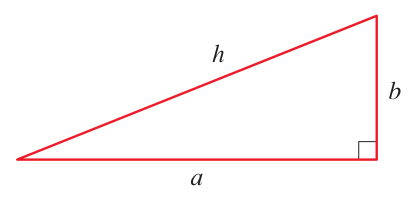
\includegraphics[height=2.3cm,keepaspectratio]{images/p0107_fig1.png}
    \end{minipage}
    \vspace{2mm}

    Để liên hệ các đại lượng đã cho với ẩn số, ta đưa vào thêm hai biến số $a$ và $b$, lần lượt là độ dài của hai cạnh góc vuông của tam giác. Điều này cho phép ta biểu diễn điều kiện đã cho, đó là tam giác vuông, bằng định lý Pytago:
    \[
    h^2 = a^2 + b^2
    \]
    Các mối liên hệ khác giữa các biến số có được bằng cách viết các biểu thức cho diện tích và chu vi:
    \[
    25 = \tfrac{1}{2}ab \qquad\qquad P = a + b + h
    \]
    Vì $P$ đã cho, lưu ý rằng lúc này ta có hệ ba phương trình với ba ẩn số $a$, $b$, và $h$:
    \begin{alignat*}{2}
        &\tikz[baseline=-0.6ex]\node[draw=stewartred,semithick,inner sep=1.5pt,rounded corners=0.5pt]{\footnotesize\textsf{\textbf{\color{stewartred}1}}};\qquad\qquad\qquad\quad & h^2 &= a^2 + b^2 \\[1.5mm]
        &\tikz[baseline=-0.6ex]\node[draw=stewartred,semithick,inner sep=1.5pt,rounded corners=0.5pt]{\footnotesize\textsf{\textbf{\color{stewartred}2}}};\qquad\qquad\qquad\quad & 25 &= \tfrac{1}{2}ab \\[1.5mm]
        &\tikz[baseline=-0.6ex]\node[draw=stewartred,semithick,inner sep=1.5pt,rounded corners=0.5pt]{\footnotesize\textsf{\textbf{\color{stewartred}3}}};\qquad\qquad\qquad\quad & P &= a + b + h
    \end{alignat*}

    Mặc dù ta có đủ số lượng phương trình, nhưng chúng không dễ để giải theo cách thông thường. Nhưng nếu ta vận dụng chiến lược giải quyết vấn đề là cố gắng nhận dạng một điều gì đó quen thuộc, ta có thể giải hệ phương trình này bằng một phương pháp dễ dàng hơn. Hãy quan sát vế phải của các Phương trình 1, 2 và 3. Những biểu thức này có gợi nhớ cho bạn điều gì quen thuộc không? Hãy chú ý rằng chúng chứa các thành phần của một hằng đẳng thức quen thuộc:
    \[
    (a + b)^2 = a^2 + 2ab + b^2
    \]
    Vận dụng ý tưởng này, ta biểu diễn $(a + b)^2$ theo hai cách khác nhau. Từ các Phương trình 1 và 2 ta có:
    \[
    (a + b)^2 = (a^2 + b^2) + 2ab = h^2 + 4(25) = h^2 + 100
    \]
    Từ Phương trình 3 ta có:
    \[
    (a + b)^2 = (P - h)^2 = P^2 - 2Ph + h^2
    \]
    \begin{align*}
        \text{\makebox[0pt][l]{\hspace{-3.2cm}Do đó}} h^2 + 100 &= P^2 - 2Ph + h^2 \\[1mm]
        2Ph &= P^2 - 100 \\[1.5mm]
        h &= \frac{P^2 - 100}{2P}
    \end{align*}
    Đây chính là biểu thức cần tìm của $h$ theo hàm số của $P$.\hfill{\color{stewartcyan}$\blacksquare$}

    \bigskip
    Như ví dụ tiếp theo minh họa, việc áp dụng nguyên tắc giải quyết vấn đề \emph{xét các trường hợp} thường là cần thiết khi xử lý các biểu thức chứa giá trị tuyệt đối.
\end{minipage}